\documentclass[10pt]{article}

\usepackage{mathtools}  % need for math tools
\usepackage{amsmath}    % need for subequations
\usepackage{graphicx}   % need for figures
\usepackage{verbatim}   % useful for program listings
\usepackage{color}      % use if color is used in text
\usepackage{subfigure}  % use for side-by-side figures
\usepackage{hyperref}   % use for hypertext links, including those to external documents and URLs
\usepackage{graphicx}   % Used to import the graphics
\usepackage{subfig}     % Used to creat subfigs

\setlength{\baselineskip}{16.0pt}   
\setlength{\parskip}{3pt plus 2pt}
\setlength{\parindent}{20pt}
\setlength{\oddsidemargin}{0.5cm}
\setlength{\evensidemargin}{0.5cm}
\setlength{\marginparsep}{0.75cm}
\setlength{\marginparwidth}{2.5cm}
\setlength{\marginparpush}{1.0cm}
\setlength{\textwidth}{150mm}



\begin{document}

\begin{center}
{\large Ay190: Computational Astrophysics (Winter Term 2012)} \\
{\large HomeWork - 6 } \\
\copyright 2012 by Arya Farahi \\
Jan 26, 2012
\end{center}

\section{Exercise 1. Solving Large Linear Systems of Equation}

Build-in : 10 S \\
Gaussian elimination : 182 S \\
Using NumPy : 7.52 S

\pagebreak

\section{Exercise 2. Root Finding: Eccentricity Anomality}

\bfseries{Part a : } \\ \mdseries
The analytical answer for this problem is:

\begin{equation}
 Y_1 = \frac{e^{100t}}{100} + \frac{99}{100}
\end{equation}

and \\

\begin{equation}
 Y_2 = - \frac{e^{100t}}{100} + \frac{1}{100}
\end{equation}

\bfseries{Part b :}\\ \mdseries

\begin{figure}[hbt]
  \centering
 \subfloat[Y1 in different grid size]{ \label{fig:1} 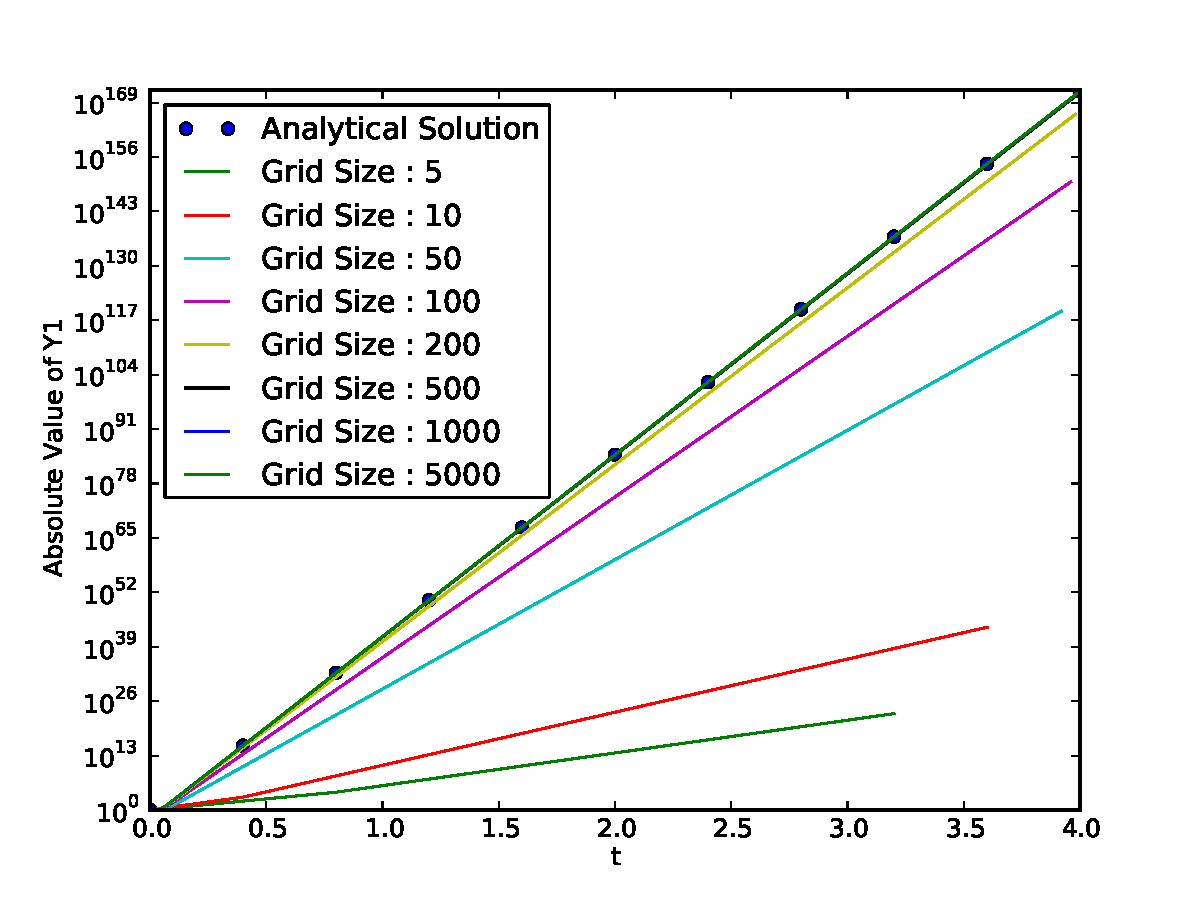
\includegraphics[scale=0.4]{Plots/plot1.pdf}}
 \subfloat[Y2 in different grid size]{ \label{fig:2} 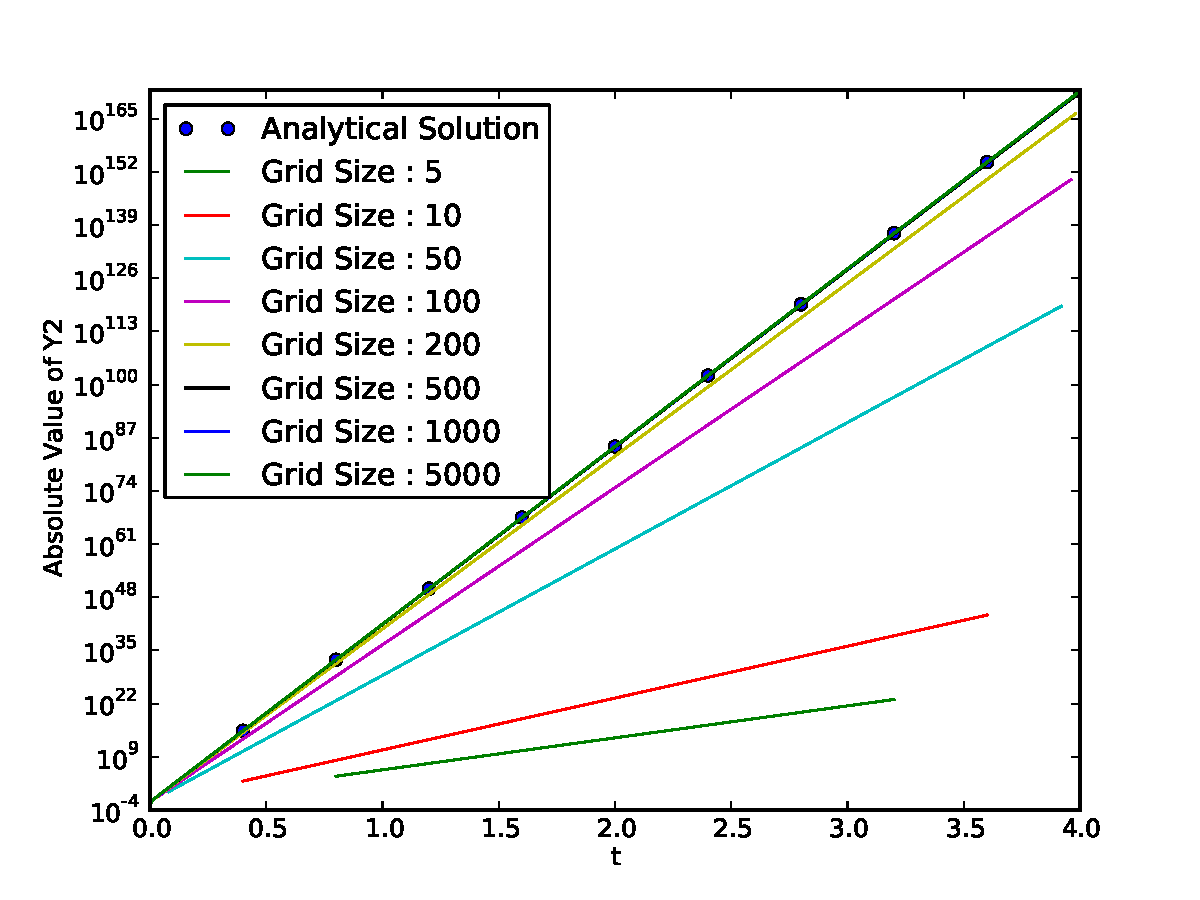
\includegraphics[scale=0.4]{Plots/plot2.pdf}}
    \caption{ Plot of Y1 and Y2 in different grid size .}
\end{figure}

\begin{figure}[hbt]
 \centering
 \label{fig:3} 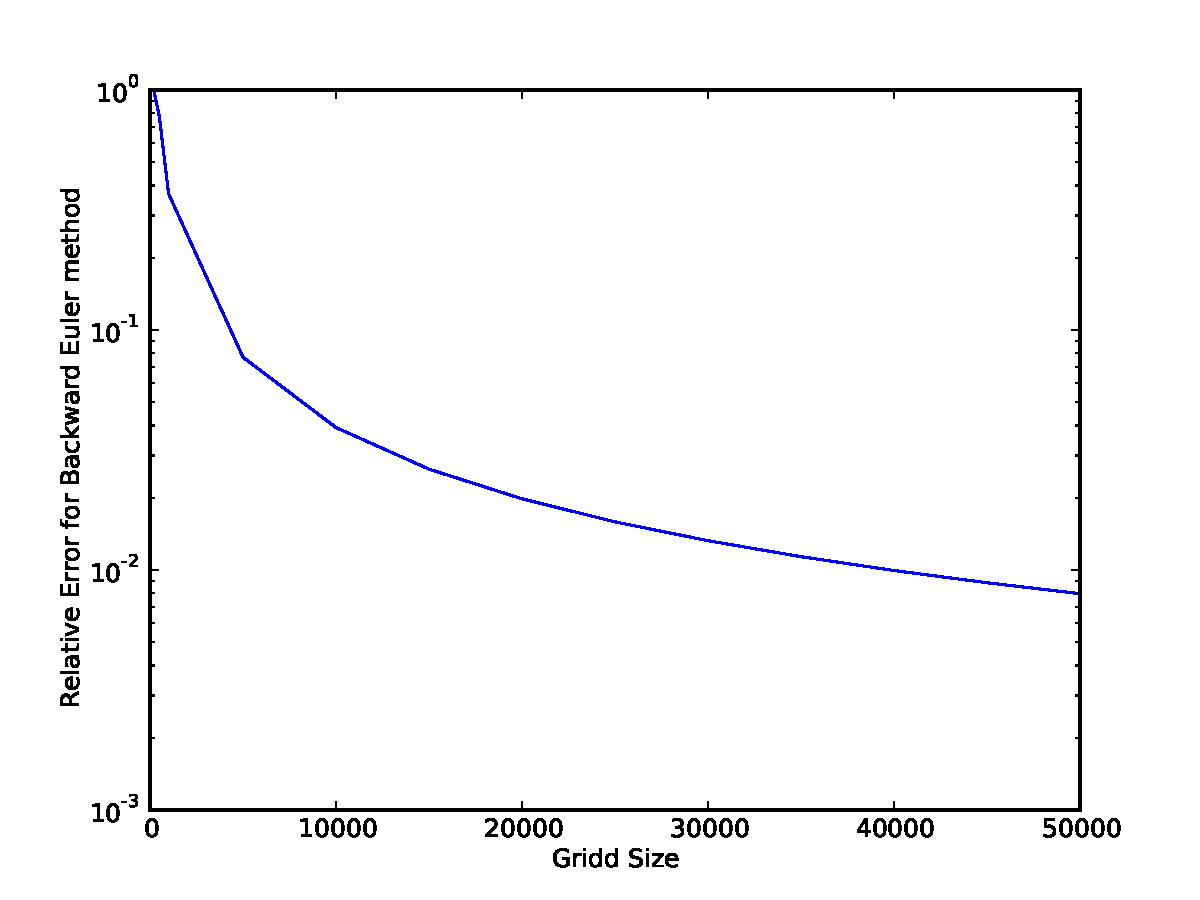
\includegraphics[scale=0.4]{Plots/plot3.pdf}
 \caption{ Plot of Relative error with increasing the grid size.}
\end{figure}


Figure \ref{fig:1} and \ref{fig:2} shows absolute value of $Y_1$ and $Y_2$ for some different grid sizes and analytical solution. Figure \ref{fig:3} showes how the relative error changing the grid size. All of this figures are the solution of out differential equation with RK4 method. \\


\bfseries{Part c :}\\ \mdseries

\begin{figure}[hbt]
  \centering
 \subfloat[Y1 in different grid size]{ \label{fig:4} 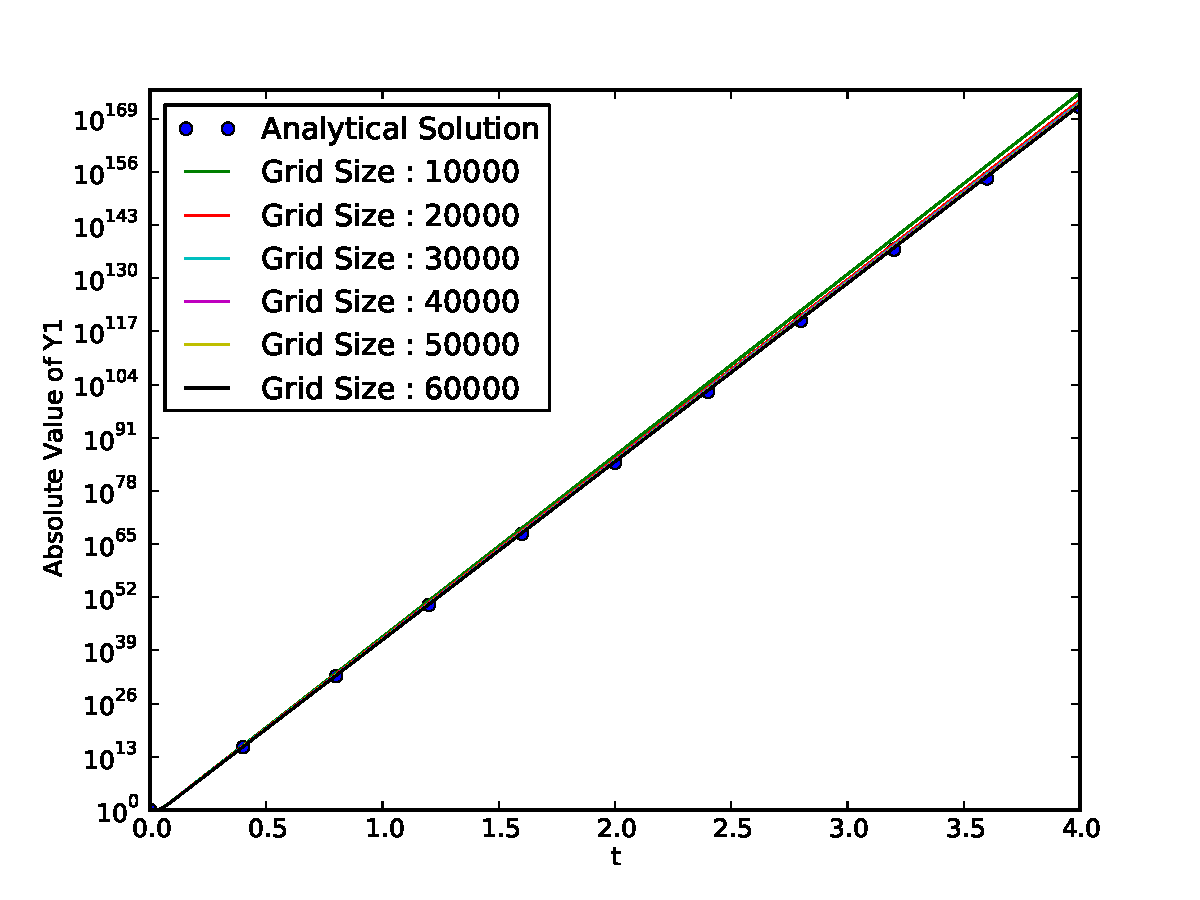
\includegraphics[scale=0.4]{Plots/plot4.pdf}}
 \subfloat[Y2 in different grid size]{ \label{fig:5} 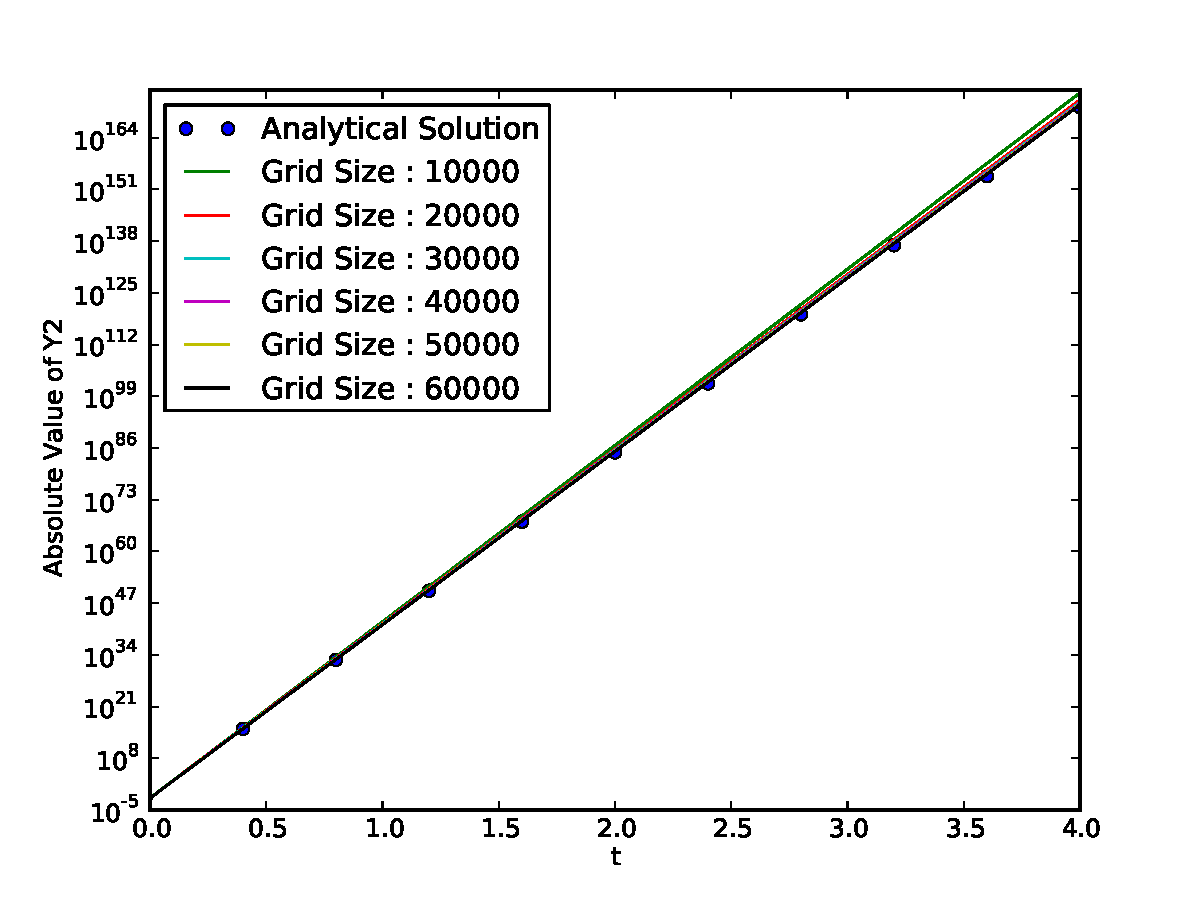
\includegraphics[scale=0.4]{Plots/plot5.pdf}}
    \caption{ Plot of Y1 and Y2 in different grid size .}
\end{figure}

\begin{figure}[hbt]
 \centering
 \label{fig:6} 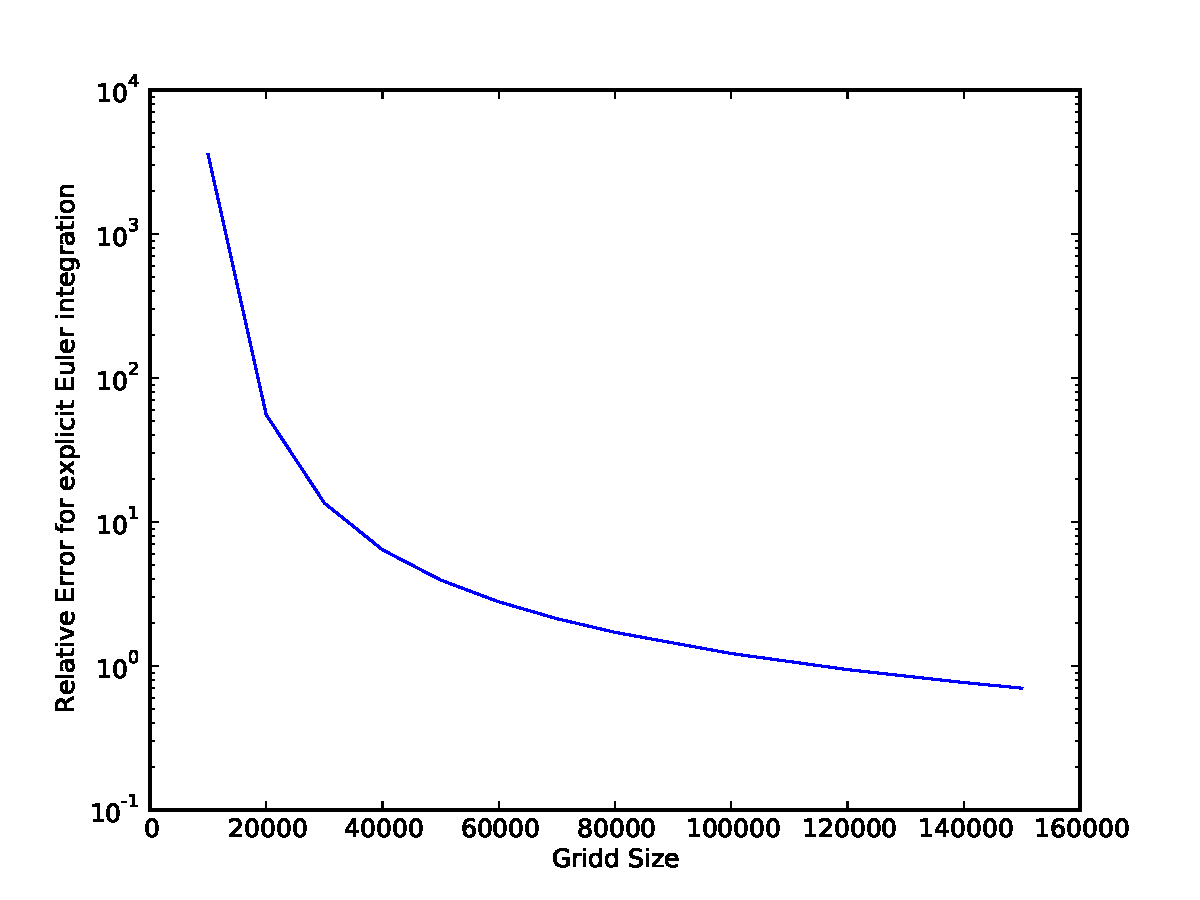
\includegraphics[scale=0.4]{Plots/plot6.pdf}
 \caption{ Plot of Relative error with increasing the grid size.}
\end{figure}

In this part I have used backward Euler method for finding the numerical answer of our problem. the final equations for this part are:\\

\begin{equation}
 Y_1^{i+1} = - \frac{(1-99dt)Y_1^i - 99dt \times Y_2^i}{1 - 100dt}
\end{equation}

and 

\begin{equation}
 Y_2^{i+1} = - \frac{ - dt \times Y_1^i - (1- dt) Y_2^i}{1 - 100dt}
\end{equation}

Figure \ref{fig:4} and \ref{fig:5} shows absolute value of $Y_1$ and $Y_2$ for some different grid sizes and analytical solution. Figure \ref{fig:6} showes how the relative error changing the grid size. All of this figures are the solution of out differential equation with back Euler method. Note that for grid size less that 400 our answer would be unstable so if we want to use this method we neet to use grid sizes more than 400. \\ 

Conclusion: \\
In conclusion based on the relative errors the KR4 method works better for this problem.
\end{document}
